\documentclass[10pt,openany]{book}

\usepackage[]{graphicx}
\usepackage[]{color}
\usepackage{alltt}
\usepackage[T1]{fontenc}
\usepackage[utf8]{inputenc}
\usepackage{array}

\newcolumntype{L}[1]{>{\raggedright\arraybackslash}p{#1}}
\newcolumntype{C}[1]{>{\centering\arraybackslash}p{#1}}
\newcolumntype{R}[1]{>{\raggedleft\arraybackslash}p{#1}}

\setcounter{secnumdepth}{3}
\setcounter{tocdepth}{3}
\setlength{\parskip}{\smallskipamount}
\setlength{\parindent}{0pt}

% Set page margins
\usepackage[top=100pt,bottom=100pt,left=68pt,right=66pt]{geometry}

% Package used for placeholder text
\usepackage{lipsum}

% Prevents LaTeX from filling out a page to the bottom
\raggedbottom

% All page numbers positioned at the bottom of the page
\usepackage{fancyhdr}
\fancyhf{} % clear all header and footers
\fancyfoot[C]{\thepage}
\renewcommand{\headrulewidth}{0pt} % remove the header rule
\pagestyle{fancy}

% Changes the style of chapter headings
\usepackage{titlesec}
\titleformat{\chapter}
   {\normalfont\LARGE\bfseries}{\thechapter.}{1em}{}
% Change distance between chapter header and text
\titlespacing{\chapter}{0pt}{50pt}{2\baselineskip}

% Adds table captions above the table per default
\usepackage{float}
\floatstyle{plaintop}
\restylefloat{table}

% Adds space between caption and table
\usepackage[tableposition=top]{caption}

% Adds hyperlinks to references and ToC
\usepackage{hyperref}
\hypersetup{hidelinks,
            linkcolor = black} % Changes the link color to black and hides the hideous red border that usually is created

% If multiple images are to be added, a folder (path) with all the images can be added here 
\graphicspath{ {images/} }

% Separates the first part of the report/thesis in Roman numerals
\frontmatter

%%%%%%%%%%%%%%%%%%%%%%%%%%%%%% Starts the document
\begin{document}

%%%%% Adds the title page
\begin{titlepage}
    \clearpage
    \thispagestyle{empty}
	\centering
	\vspace{2cm}

    % Titles
    % Information about the University
	{\normalsize  Computer Science and Engineering\\Software Engineering 2 Project - Prof. Elisabetta Di Nitto\par}
	\vspace{3cm}
	{\Huge \textbf{CLup – Customers Line-up}} \\
	\vspace{1cm}
	{\large \textbf{Requirement Analysis and Specification
    Document} \par}
	\vspace{4cm}
	{\normalsize Marco Di Gennaro (10596841)\\Luca Danelutti (10604455)  \par}
	\vspace{2cm}

    
\includegraphics[scale=0.4]{images/Logo_Politecnico_Milano.png}
    
    \vspace{2cm}

	% Set the date
	{\normalsize December 23, 2020 \par}
	
	\pagebreak

\end{titlepage}

% Adds a table of contents
\tableofcontents{}

\clearpage

%%%%%%%%%%%%%%%%%%%%%%%%%%%%%%%%%%%%%%%%%%%%%%%%%%%%%%%%%%%%%%%%%%%%%%%%%%%%%%%%%%%%%%%%%%%%
%%%%%%%%%%%%%%%%%%%%%%%%%%%%%%%%%%%%%%%%%%%%%%%%%%%%%%%%%%%%%%%%%%%%%%%%%%%%%%%%%%%%%%%%%%%%
%%%%% Text body starts here!
\mainmatter

\chapter{Introduction}

	\section{Purpose}

		This document represents the Requirement Analysis and Specification Document (RASD).
It contains the description of the main goals, the domain and its representation through some models, the uses cases that describe the scenario, the list of functional and non-functional requirements and specifications that characterize the software described in the following subsession.
It also includes the revision history to better understand the development of this document.
This document is addressed to the developers who will have to implement the described system and it has the purpose to guide them through the development process.

	\section{Scope}

		The system aims to provide a solution to reduce overcrowding both inside and outside grocery stores.
Due to the coronavirus emergency supermarkets need to restrict access to their stores to avoid having crowds inside, but at the same time they must avoid long queues outside which are themselves a potential risk. \newline

The application would work as a digital counterpart to the common situation where people who are in line for a service retrieve a number that gives their position in the queue.
The system should provide both the possibility to line up remotely (for example through a mobile phone) and at the grocery store for those customers who do not have access to the required technology (\textbf{Lineup functionality}).
Each customer that lined up should receive a number. Users should wait until his/her number is being called (or close to being called) to approach the store. This should reduce overcrowdings outside supermarkets.
Users can also scan a QR code when entering the grocery store, enabling the store manager to monitor entrances. \newline

In addition to lining up directly an advanced function is offered. Customers can also book a visit to the supermarket, similarly to booking a slot for visiting a museum. The system should be able to schedule customer visits correctly given that each visit will last differently from the others.  
CLup can ask the customer details about his/her visit or it can compute an estimated duration from previous visits of the same user (\textbf{Book a visit functionality}). \newline

Ultimately, the system will have to be easy-to-use given that everyone needs to do grocery shopping and the more users will use the system remotely the more CLup will be effective.

\subsection{World Phenomena} %Customer/A customer
\begin{center}
    {\renewcommand{\arraystretch}{2}%
    \begin{tabular}{L{2cm}L{12cm}}
        \hline
        \textbf{WP1} & Customer wants to go grocery shopping at that time \\
        \hline
        \textbf{WP2} & Customer wants to go grocery shopping in the future \\
        \hline
        \textbf{WP3} & Customer wants to line up \\
        \hline
        \textbf{WP4} & Customer wants to book a visit in the future \\
        \hline
        \textbf{WP5} & Customer goes to the supermarket and he/she has a booking/lined up \\
        \hline
        \textbf{WP6} & Customer goes to the supermarket and he/she does not have a booking/didn't line up \\
        \hline
        \textbf{WP7} & Grocery store has a limited capacity due to the Covid19 restrictions \\
        \hline
        \textbf{WP8} & The store manager wants to monitor and control entries in his/her store \\
        \hline
    \end{tabular}}
\end{center}

\subsection{Shared Phenomena}
\begin{center}
    {\renewcommand{\arraystretch}{2}%
    \begin{tabular}{L{2cm}L{12cm}}
        \hline
        \textbf{SP1} & Customer books a visit \\
        \hline
        \textbf{SP2} & Customer specifies what he/she will buy (or the shop departments he/she will mostly go to) in his/her next visit \\
        \hline
        \textbf{SP3} & Customer lines up remotely \\
        \hline
        \textbf{SP4} & Customer lines up at the grocery store \\
        \hline
        \textbf{SP5} & Customer is called by the CLup system \\
        \hline
        \textbf{SP6} & Customer shows his/her number entering the store \\
        \hline
        \textbf{SP7} & Customer shows his/her QR Code entering the store \\
        \hline
        \textbf{SP8} & Customer shows his/her visit booking entering the store \\
    \end{tabular}}
\end{center}

\subsection{Goals}
\begin{center}
    {\renewcommand{\arraystretch}{2}%
    \begin{tabular}{L{2cm}L{12cm}}
        \hline
        \textbf{G1} & All customers who reserve a place in the queue must be able to enter the supermarket \\
        \hline
        \textbf{G2} & Allow customers to enter the store once their number has been called or if they have booked a visit for that time slot \\
        \hline
        \textbf{G3} & Customers who go to the supermarket without a number/booking are allowed to line up at the store \\
        \hline
        \textbf{G4} & Inside the grocery store it must be feasible to follow Covid19 regulations \\
        \hline
        \textbf{G5} & Outside the grocery store there must not be long queues or overcrowding \\
        \hline
        \textbf{G6} & Customer is allowed to book a visit through the CLup system \\
        \hline
        \textbf{G7} & Customer is allowed to line up through the CLup system \\
        \hline
        \textbf{G8} & The store manager is allowed to control entrances to his/her store \\
        \hline
        \textbf{G9} & The store manager is allowed to monitor entrances of customers that used the QR Code \\
        \hline
        \textbf{G10} & Customer is allowed to approach the store in time with respect to his position in the queue \\
        \hline
    \end{tabular}}
\end{center}

	\section{Definitions, Acronyms, Abbreviations}

		\subsection{Definitions}

\subsection{Acronyms}

\subsection{Abbreviations}

	\section{Revision history}

		\begin{center}
    {\renewcommand{\arraystretch}{2.4}%
    \begin{tabular}{L{2cm}L{14cm}}
        \hline
        \textbf{Date} & \textbf{Description} \\
        \hline
        ? & ? \\
        \hline
    \end{tabular}}
\end{center}

	\section{Reference Documents}

		\begin{itemize}
    \item Specification Document : "R\&DD Assignment AY 2020-2021"
    \item Lecture slides
\end{itemize}

	\section{Document Structure}

		This document is composed of six chapters :
\begin{itemize}
    \item \textbf{Chapter 1: Introduction.} This chapter includes the goals of the project (\textit{Purpose}) 
    and an analysis of the world and the shared phenomena (\textit{Scope}). It also includes a section where 
    there are all the descriptions, acronyms, and abbreviations in the document. Lastly, there 
    is a revision history and a reference documents list
    \item \textbf{Chapter 2: Overall Description.} This chapter includes scenarios and further
    details on the shared phenomena and a domain model (class diagrams and statecharts) (\textit{Product perspective}). It also
    shows the most important requirements (\textit{Product functions}). It clarifies the user needs (\textit{User charateristics}), and lastly, it contains 
    the domain assumptions (\textit{Assumptions, dependencies and constraints})
    \item \textbf{Chapter 3: Specific Description.} This chapter is the body of the documents. It includes a section for 
    the User, Hardware, Software, and Communication Interfaces (\textit{External Interface Requirements}). It also contains a definition
    of use case diagrams, use cases, and associated sequence/activity diagrams, and a map on requirements (\textit{Functional Requirements}).
    Lastly, there are three sections dedicated to non-functional requirements (\textit{Performance Requirements}, \textit{Design Constraints} \textit{Software System Attributes})
    \item \textbf{Chapter 4: Formal Analysis Using Alloy.} This chapter includes a brief presentation of the
    main objectives driving the formal modeling activity, as well as a description of the model.
    itself, what can be proved with it, and why what is proved is important given the problem at hand. It also includes some worlds obtained by running the
    formal model and the results of the checks performed on the meaningful assertion
    \item \textbf{Chapter 5: Effort Spent.}  This chapter includes information about the number of hours each group member has worked for this document
    \item \textbf{Chapter 6: References.}
\end{itemize}

\chapter{Overall Description}\label{chapt:sum}

	\section{Product perspective}

		Here is the application domain model of this project. In particular, this section focuses on the object model (\textbf{static information models} and \textbf{dynamic class behaviour models}).
\subsection{Static Information Model}
The below high-level diagram provides a static information model of the application domain. Basically, it is the structure of the world, it contains only few attributes, and it doesn't include every class that will be necessary to define the model of the CLup system. \newline

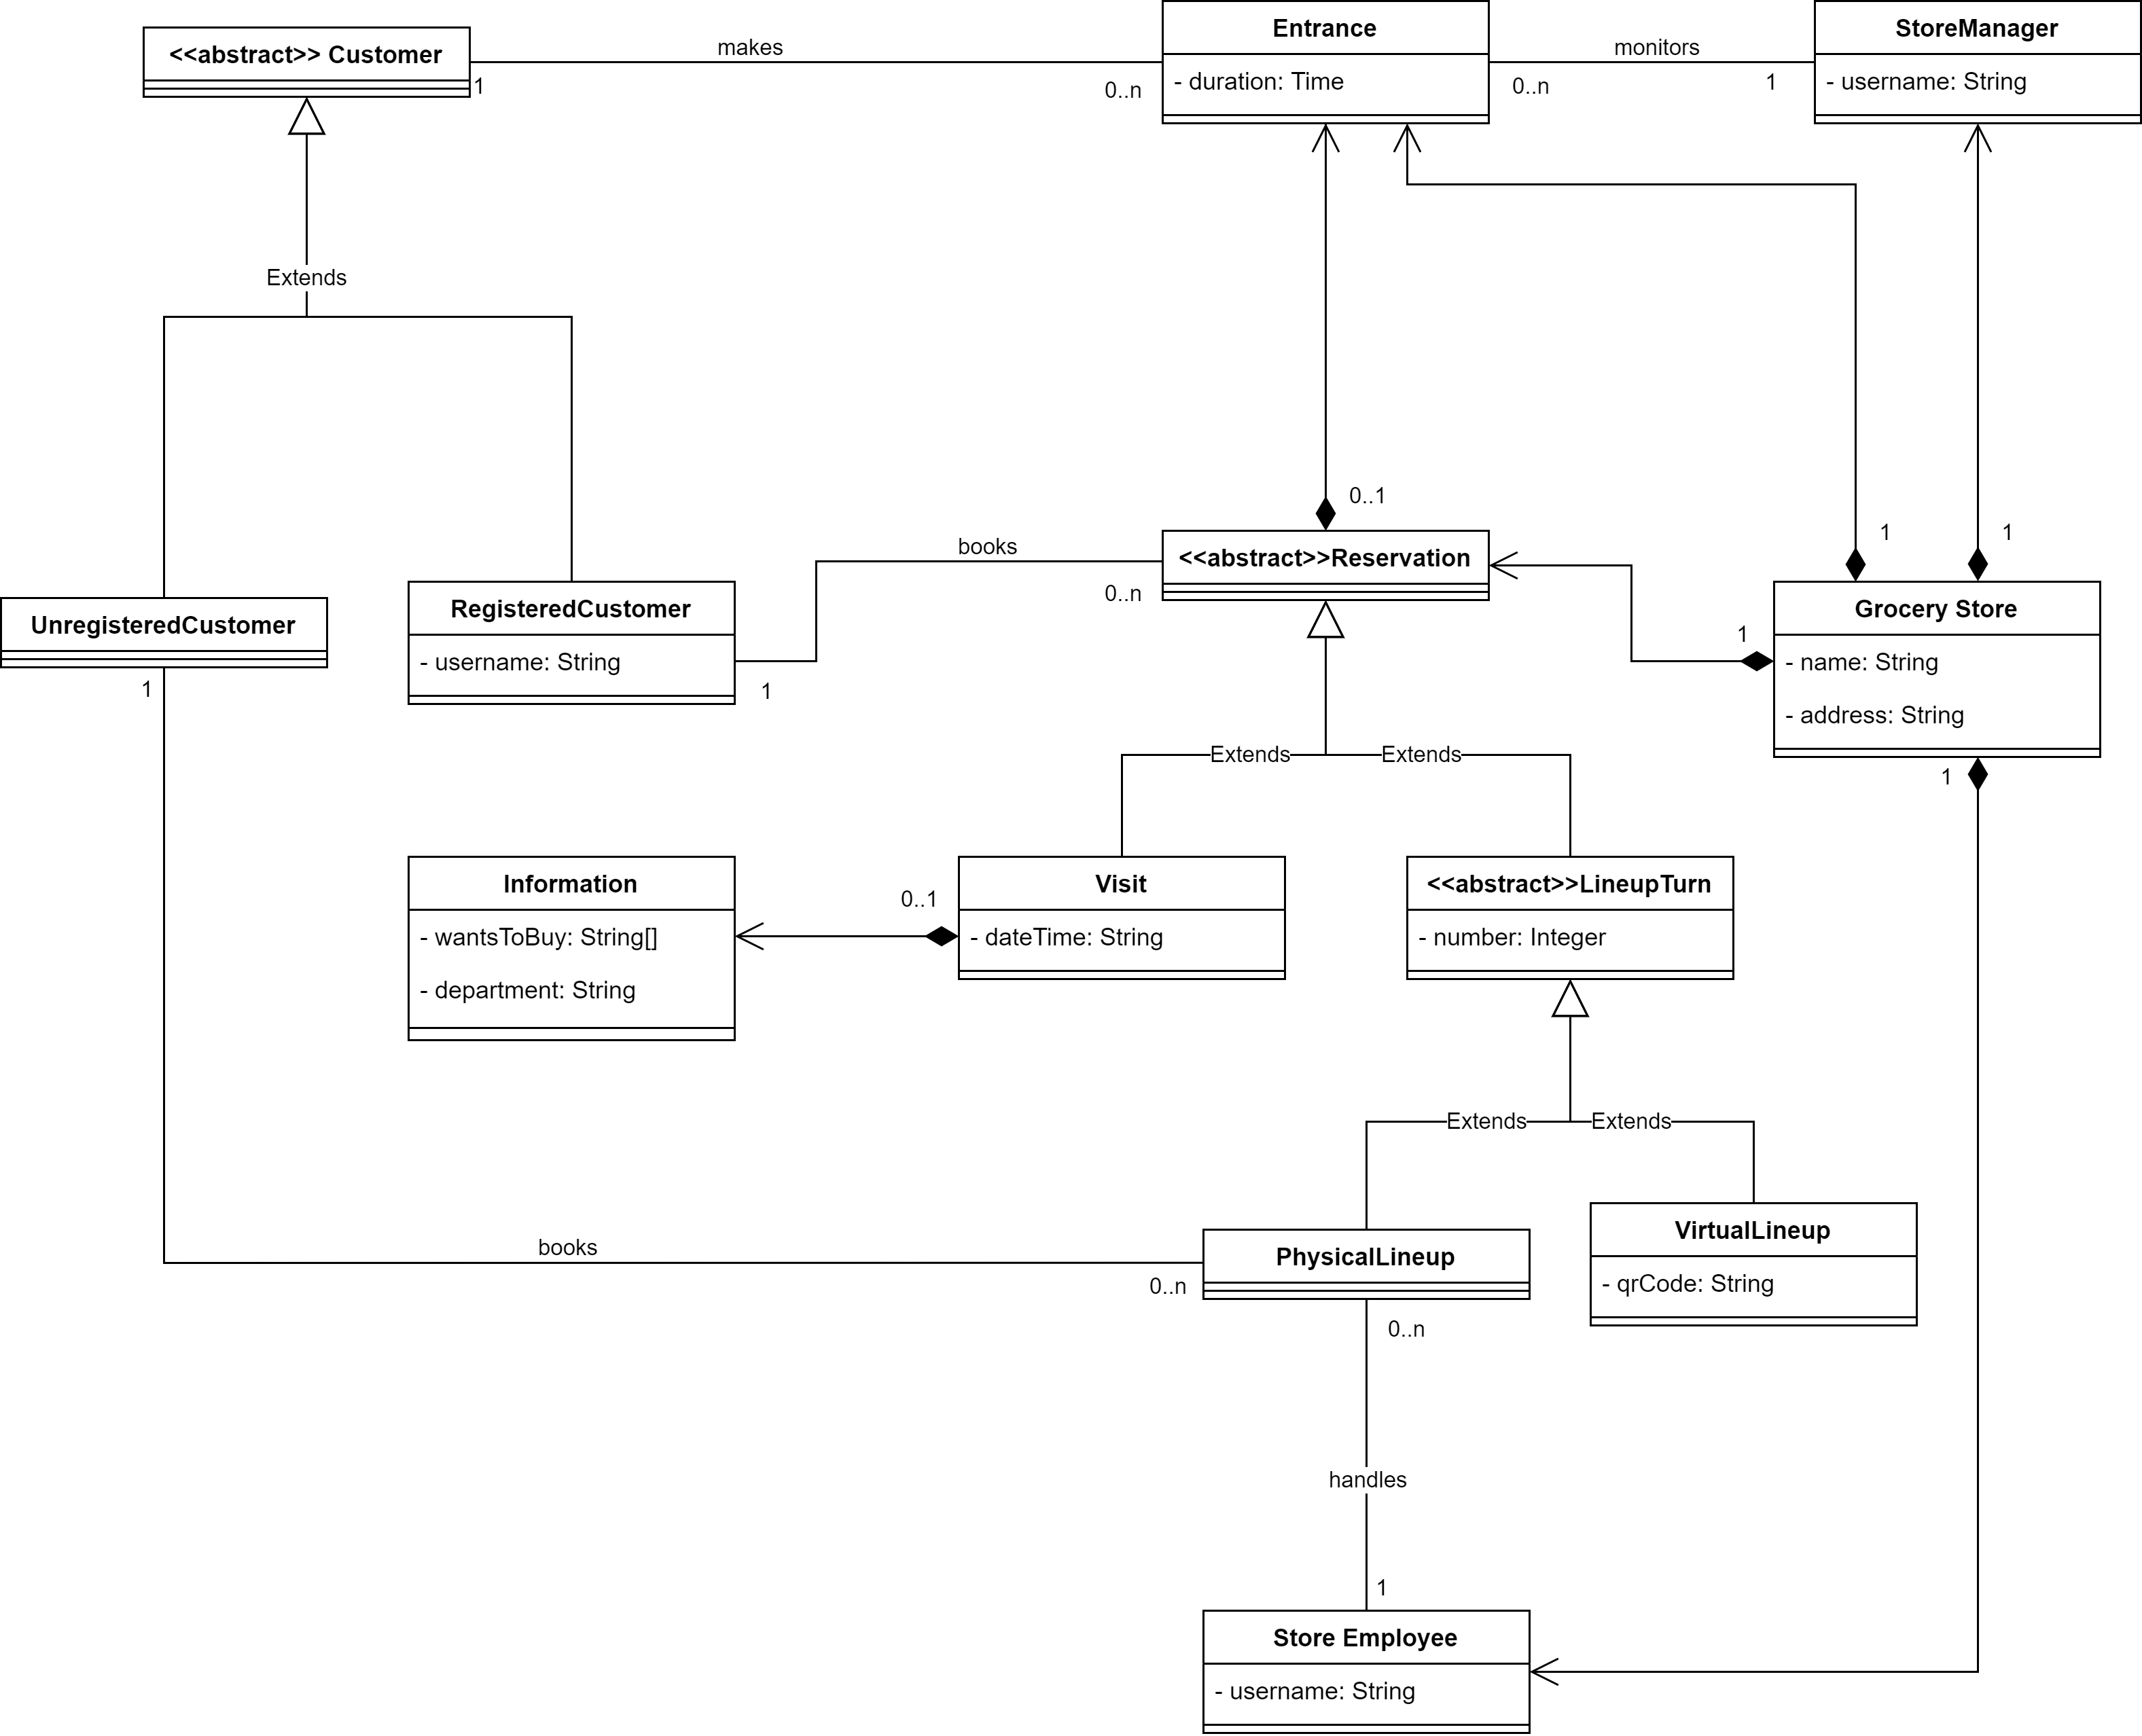
\includegraphics[width=\textwidth]{class_diagram.png}


\subsection{Dynamic Class Behaviour Models}
The below state diagrams shows some	critical aspects of	the	application, how the behaviour of these critical aspects is modeled and the evolution of their states.

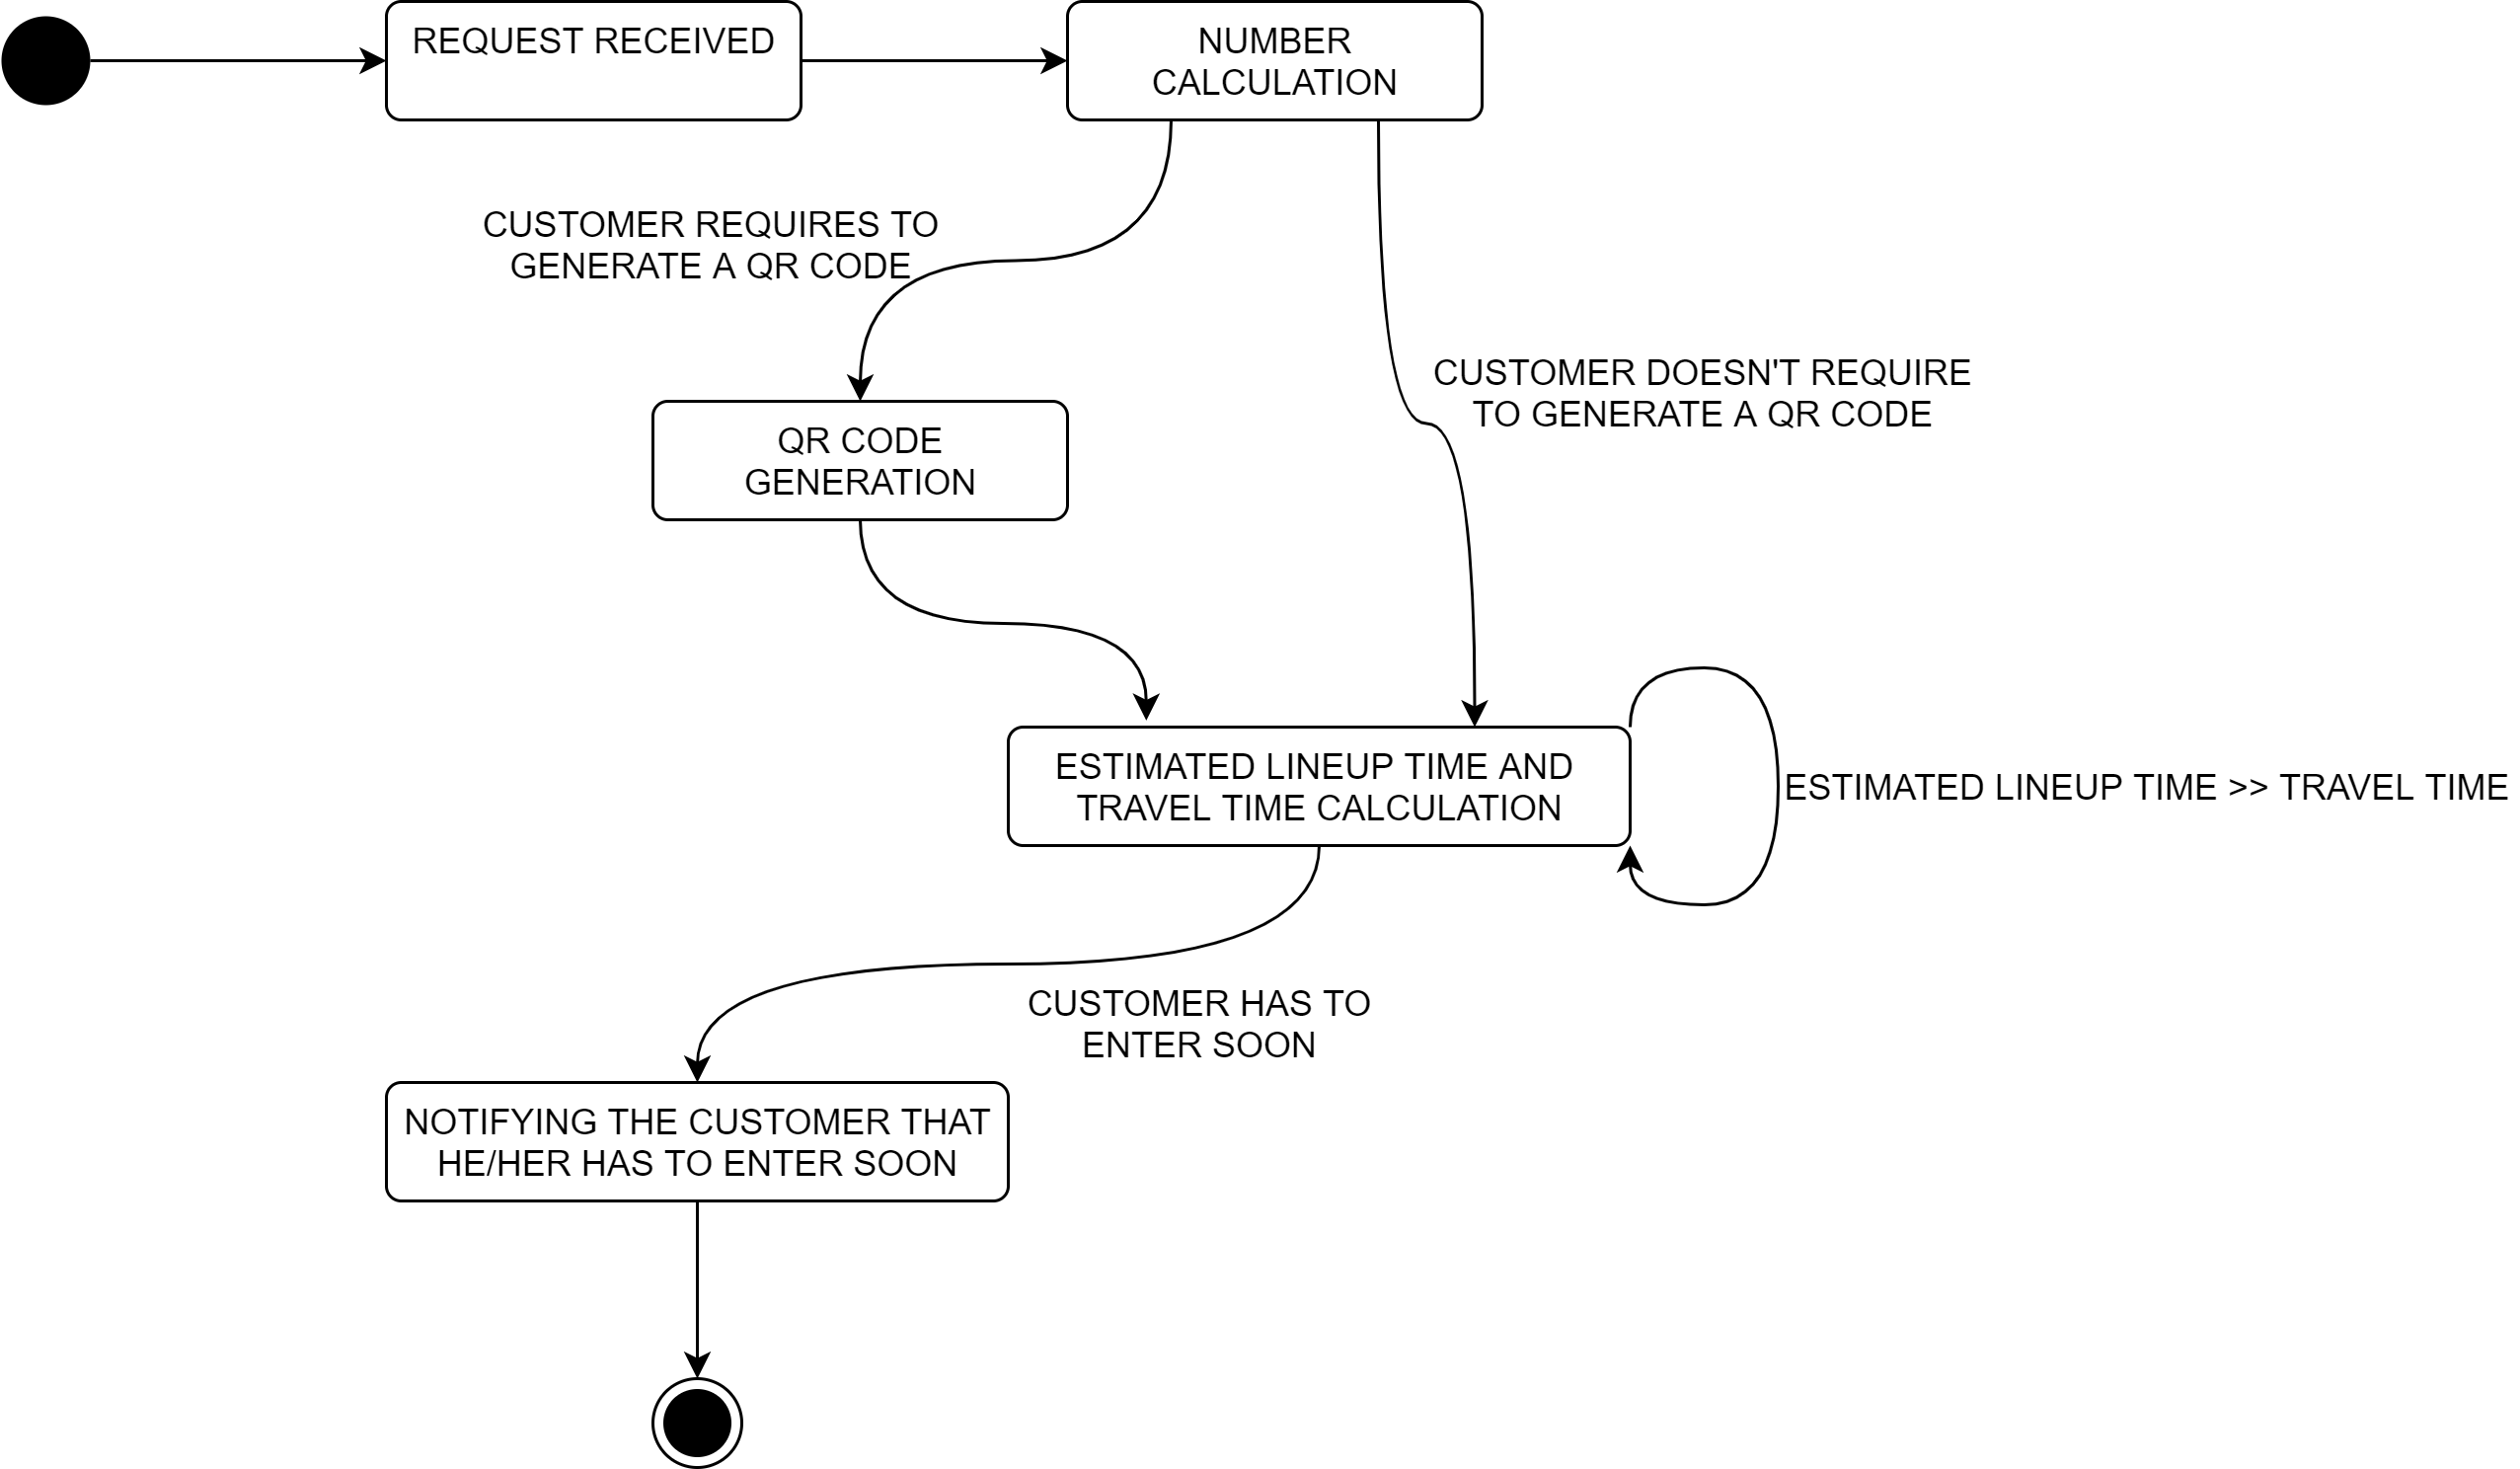
\includegraphics[width=\textwidth]{state_diagram1.png}

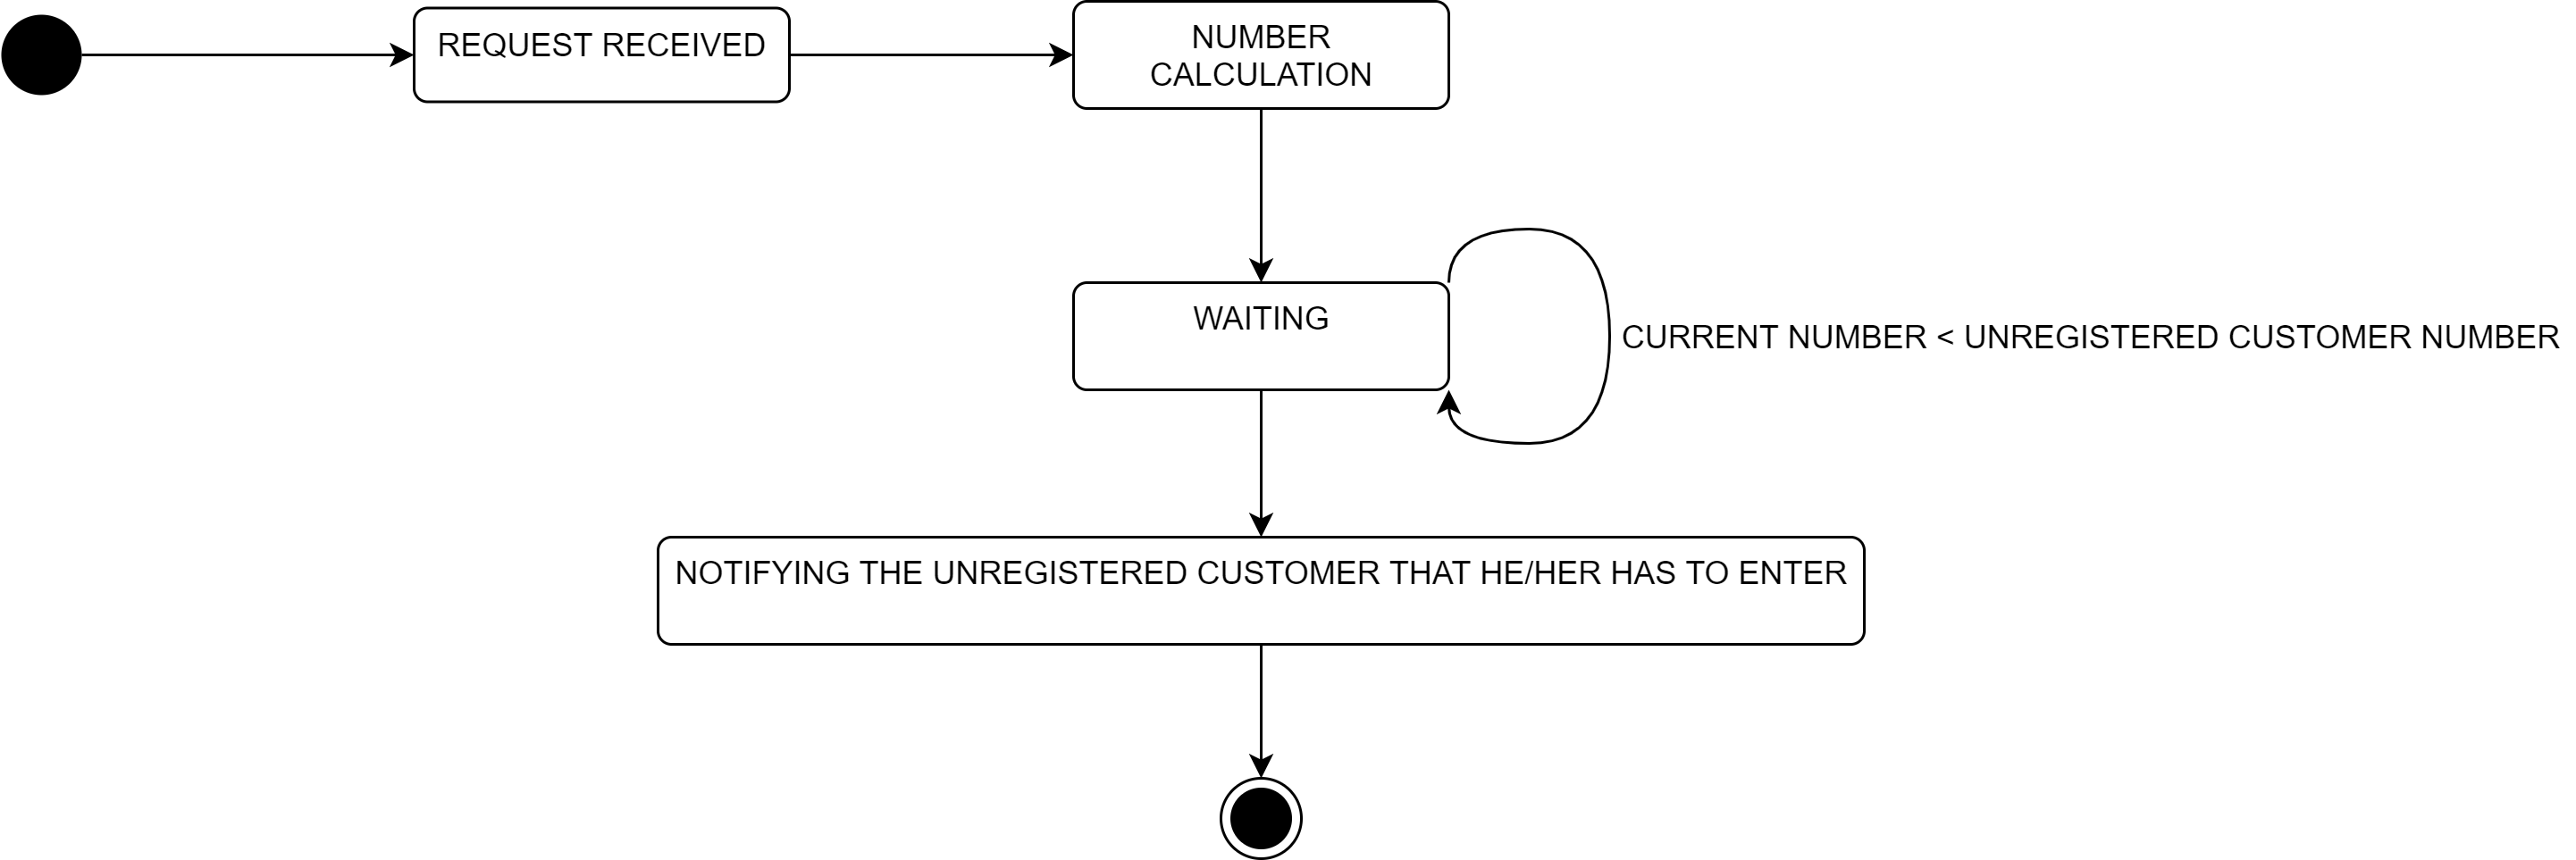
\includegraphics[width=\textwidth]{state_diagram2.png}

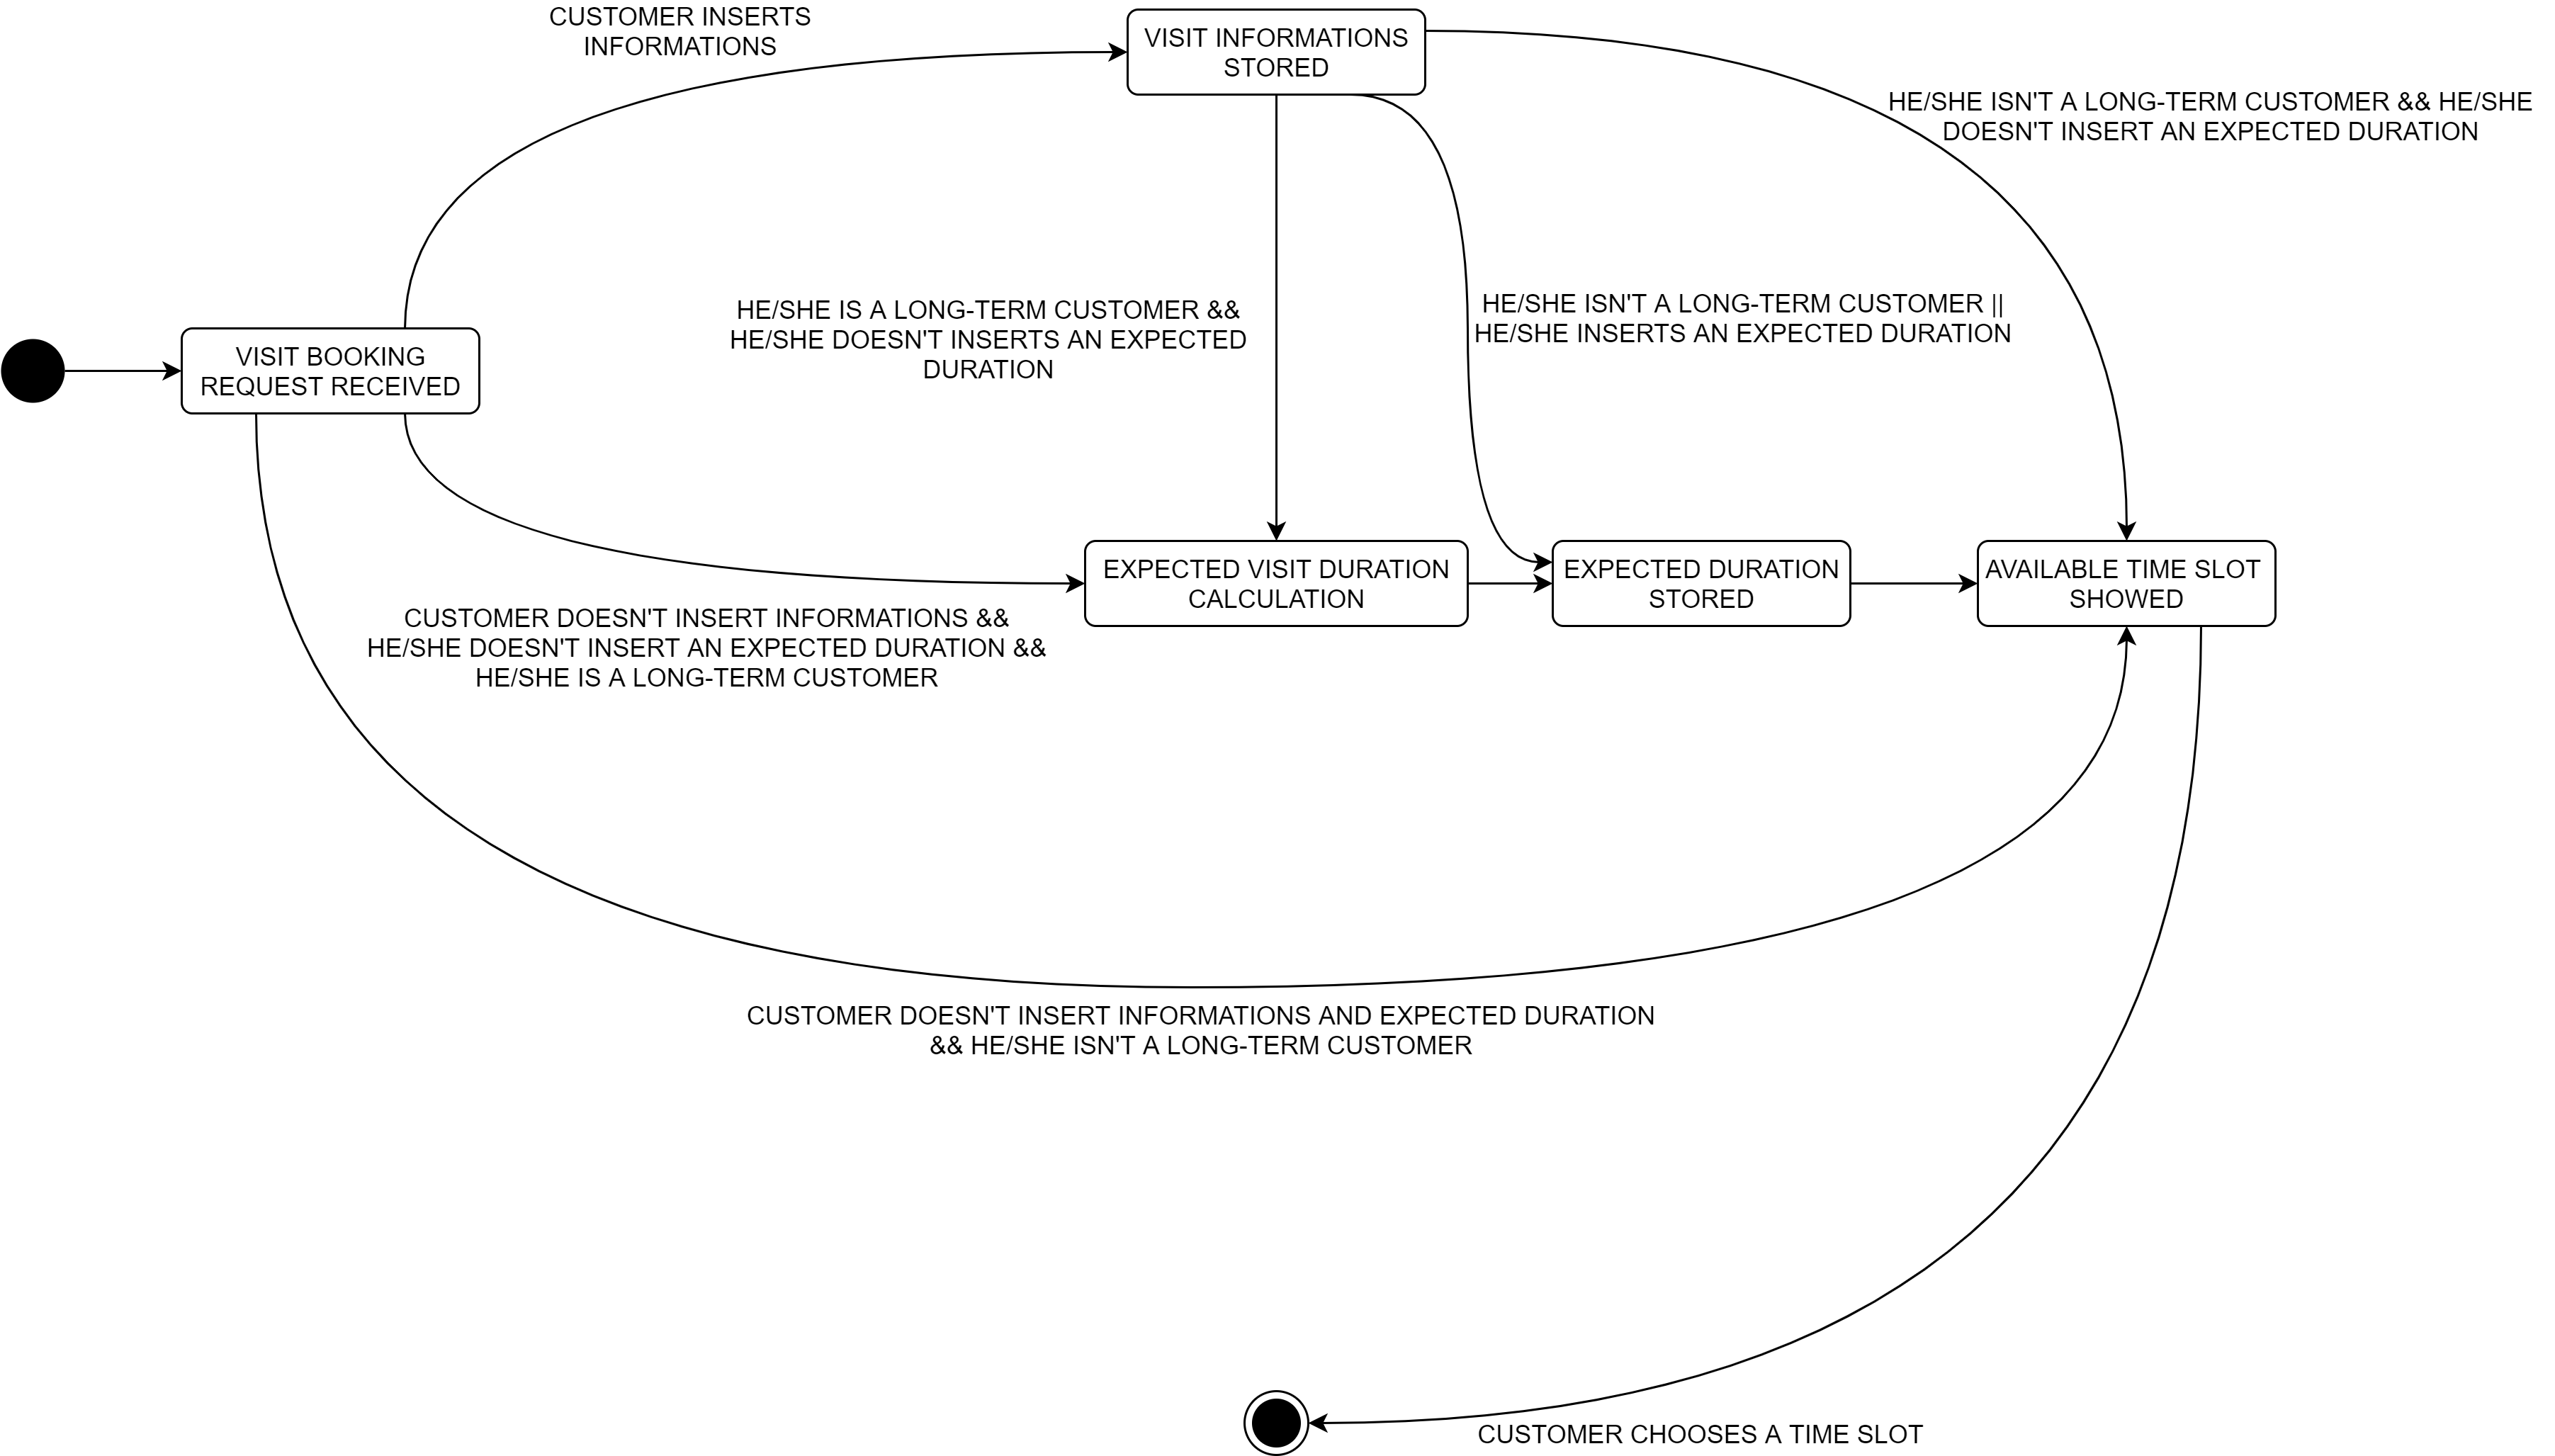
\includegraphics[width=\textwidth]{state_diagram3.png}

	\section{Product functions}

		Here is the description of the major function that CLup system has. In particular, we identified four significative function, they are :
\begin{itemize}
    \item \textbf{Reservation of a number for a line up :}
    \item \textbf{Booking a visit :}
    \item \textbf{Identification of a customer at the store entrance :}
    \item \textbf{Collection and data elaboration :}
\end{itemize}

	\section{User characteristics}

		The actors of the application are the following:
\begin{itemize}
    \item \textbf{Unregistered customer:} a person who can sign up to the CLup service. If the user doesn't have a compatible device to register to CLup he/she can go to the store and line up there.
    \item \textbf{Registered customer:} a person passed through the registration process. He/she is able to line up digitally or to book a visit right from the CLup application.
    \item \textbf{Store employee:} a person who works at a grocery store and is registered to CLup as employee. He/she can line up customers who arrived at the store without lining up digitally. He/she will then call the customers when it's time to enter the supermarket.
    \item \textbf{Store manager:} a person who works at a grocery store as the manager of that shop. He/she can manage the store informations on the CLup platform like the opening hours or the store capacity.
\end{itemize}

	\section{Assumption, dependencies and constraints}
	
		In the specification document presented by the client we found some points that lacked in precision. In order to better clarify and to make you understand better the content of this document we decided to introduce those assumptions.
\subsection{Text assumptions}
\begin{itemize}
    \item Entrances monitoring is referred to customers using their personal QR code.
    \item QR Code scanning is not mandatory: customers who will scan their QR code when entering the store will contribute to entrances monitoring, thoose who will not will not contribute to such statistics.
    \item Previous visits durations are inserted in the CLup system in some way.
\end{itemize}

\subsection{Domain assumptions}

    \begin{center}
        {\renewcommand{\arraystretch}{2}%
        \begin{tabular}{L{2cm}L{12cm}}
            \hline
            \textbf{D1} & The CLup system is enabled only when entrances control is needed \\
            \hline
            \textbf{D2} & Store has a capacity greater than 0 \\
            \hline
            \textbf{D3} & Customer who lines up has a GPS enabled device \\
            \hline
            \textbf{D4} & GPS is enabled between the line up and the departure to approach the store \\
            \hline
            \textbf{D5} & The user has a working internet connection \\
            \hline
            \textbf{D6} & The store has an available employee to serve customers who physically want to line up and retrieve a number \\
            \hline
            \textbf{D7} & The store employee who lines up customers will call them when they are allowed to enter the store \\
            \hline
            \textbf{D8} & Stores are uniquely identified \\
            \hline
            \textbf{D9} & The customer's device, the store and the CLup system have a syncronized date and time \\
            \hline
            \textbf{D10} & A QR code scanner will be available entering the store \\
            \hline
            \textbf{D11} & The store is physically accessible \\
            \hline
            \textbf{D12} & There is a route from the customer to the store \\
            \hline
            \textbf{D13} & The estimated time to enter the store is greater than the estimated time to approach the store \\
            \hline
            \textbf{D14} & The customer stay at the store is limited in time \\
            \hline
            \textbf{D15} & No two customers have the same number when entering at the same time \\
            \hline
            \textbf{D16} & The customer who specifies what he/she will buy/what departments he/she will go to will comply with his/her estimations \\
            \hline
            \textbf{D17} & Customer has a CLup compatible device \\
            \hline
            \textbf{D18} & Store has a CLup compatible device \\
            \hline
        \end{tabular}}
    \end{center}

\chapter{Specific Requirements}\label{chapt:sum}

\chapter{Formal Analysis Using Alloy}\label{chapt:sum}

\chapter{Effort Spent}\label{chapt:sum}

\chapter{References}\label{chapt:sum}

\pagebreak


% Adding a bibliography if citations are used in the report
\bibliographystyle{plain}
\bibliography{BiBTeXexempel.bib}
% Adds reference to the Bibliography in the ToC
\addcontentsline{toc}{chapter}{\bibname}

\end{document}